%%%%%%%%%%%%%%%%%%%%%
%   AMS packages    %
%%%%%%%%%%%%%%%%%%%%%
\documentclass{amsart}
\usepackage{amsmath}
\usepackage{amsxtra}
\usepackage{amscd}
\usepackage{amsthm}
\usepackage{amsfonts}
\usepackage{amssymb}
\usepackage{eucal}
\usepackage[all]{xy}
\usepackage{graphicx}
\usepackage{comment}
\usepackage{amssymb}
\usepackage{tikz-cd}
\usetikzlibrary{matrix,arrows,decorations.pathmorphing}

\newtheorem{cor}[subsubsection]{Corollary}
\newtheorem{lem}[subsubsection]{Lemma}
\newtheorem{prop}[subsubsection]{Proposition}
\newtheorem{propconstr}{Proposition-Construction}
\newtheorem{ax}{Axiom}
\newtheorem{conj}{Conjecture}
\newtheorem{thm}[subsubsection]{Theorem}
\newtheorem{defn}[subsubsection]{Definition}
\newtheorem{rem}[subsubsection]{Remark}
\newtheorem{eg}[subsubsection]{Example}
\newtheorem{ex}[subsubsection]{Exercise}
\newtheorem{note}[subsubsection]{Notation}
\newtheorem{alg}[subsubsection]{Algorithm}
\newtheorem{fact}[subsubsection]{Fact}

\newcommand\nc{\newcommand}
\nc\on{\operatorname}
\nc\renc{\renewcommand}
\newcommand\ssec{\subsection}
\newcommand\sssec{\subsubsection}
\newcommand\bO{{\mathbf O}}
\newcommand\CC{{\mathcal C}}
\newcommand\BN{{\mathbb N}}
\newcommand\BC{{\mathbb C}}
\newcommand\BF{{\mathbb F}}
\newcommand\BR{{\mathbb R}}
\newcommand\BQ{{\mathbb Q}}
\newcommand\BBZ{{\mathbb Z}}
\newcommand\uR{\underline{R}}
\newcommand\uZ{\underline{\BBZ}}
\newcommand\CF{{\mathcal F}}
\newcommand\uCF{\underline{{\mathcal F}}}
\newcommand\BZ{{\mathbb Z}}
\newcommand\BA{{\mathbb A}}
\newcommand\BP{{\mathbb P}}
\newcommand\fa{{\mathfrak a}}
\newcommand\fp{{\mathfrak p}}
\newcommand\fq{{\mathfrak q}}
\newcommand\fm{{\mathfrak m}}
\newcommand\pt{\mathrm{pt}}
\nc{\bd}{\mathbf{d}}
\nc{\Hom}{\on{Hom}}
\nc{\End}{\on{End}}
\nc{\Spec}{\on{Spec}}
\nc{\Reg}{\on{Reg}}
\nc{\Specm}{\on{Specm}}
\nc\ol{\overline}
\nc\wt{\widetilde}
\nc{\one}{{\mathbf{1}}}
\renc{\mod}{\on{-mod}}
\newcommand{\id}{\mathrm{id}}
\nc{\ul}{\underline}
\nc{\uHom}{\ul\Hom}
\nc{\tHom}{\ul\uHom}
\nc{\wh}{\widehat}
\nc{\Vect}{\on{Vect}}
\nc{\Res}{\on{Res}}
\nc{\Ind}{\on{Ind}}

\newcommand\im{\text{Im}}

\title{Unimodality Ideas}
\author{Aaron Landesman}
\usepackage{amsmath}
\begin{document}

\maketitle
\section{Directions to move}
\begin{enumerate}
	\item Look at generalising $p_i^r$ for general r.
	\item Generalizing to $q$ analog of cyclic group.
	\item Try relating $p_i,q_i.$
	\item Coding which groups $G$ we have $p_i=q_i.$
	\item When are $p_i = q_i.$
	\item Try to compute $q_i.$
	\item Look at simple groups, and maybe solvable groups, try quotienting by normal subgroups?
	\item Are there any ways to combine $G_1,G_2$ where $G_i$ are groups with $p_i = q_i.$
	\item Are there some characterisations of groups with $q_i,p_i.$
	\item How to use sage, what can we do with groups?
	\item Which edge poset definition do we want? Do we include edges containing $y$ or exclude them?
	\item Look at $B_n(q).$ 
	\item Look at generalizing $F_r(B_n)$ to arbitrary posets
	\item Try relating Wilson's Normal Form to our posets?
\end{enumerate}

\section{The Functor of Faces}
\begin{rem}
We assume all posets are ranked posets, and $G$ actions are rank preserving, order preserving actions.
\end{rem}

\begin{defn}
Define the poset category $\mathcal P_r,$ where the objects $P \in \mathcal P_r$ are ranked poset, and the morphisms $Mor(P,Q)$ are rank preserving, order preserving maps, which send all $B_{r+1}$ to other $B_{r+1}$.
\end{defn}

\begin{defn}
Define the {\it Functor of Faces} $\mathcal F:\mathcal P \rightarrow \mathcal P,$ that associates to any poset $P \in \mathcal P$ a poset $\mathcal F(P),$ where the vertices of $\mathcal F(P)$ are pairs $(x,y)\in P \times P,x \lessdot y,$ and the ordering in $\mathcal F(P)$ is given by $(x,y)\leq (a,b)$ if $x \leq a,y\leq b.$ For $f \in Mor(P,Q),$ the corresponding morphism $\mathcal F(f):\mathcal F(P) \rightarrow \mathcal F(Q),$ given by $\mathcal F(f)(x,y) = (f(x),f(y)).$
\end{defn}

\begin{conj}
The Functor of faces $\mathcal F$ is fully faithful.
\end{conj}

\section{Quotient Edges}

This section will build up to the theorem that for a symmetric poset $P,$ with $\mathcal F(P)$ having injective order raising maps for rank $i < \frac{n}{2}$, we will also have $\mathcal F(P/G)$ has injective order raising maps for $i < \frac{n-1}{2}.$ 

\begin{note}
Let $U_i:P_i \rightarrow P_{i+1}$ be the raising operator for the poset $P.$ Then, we obtain an induced map
\begin{align*}
	U_i \otimes U_{i+1}:P_i\otimes P_{i+1} \rightarrow P_{i+1} \otimes P_{i+1},x \otimes y \mapsto U(x) \otimes U(y).
\end{align*}
\end{note}

\begin{note}
We also have the natural inclusions
\begin{align*}
	k_i:\mathcal F(P)_i &\rightarrow P_i \otimes P_{i+1},\\
	x\otimes y &\mapsto x\otimes y\\
	k_i^{G\times G}:\mathcal F(P/G)_i &\rightarrow (P/G)_i \otimes (P/G)_{i+1},\\
	Gx\otimes Gy &\mapsto Gx\otimes Gy,
\end{align*}
where we have $x \lessdot y$ and $Gx \lessdot Gy.$ The maps above are defined on a basis, and are extended by linearity.
\end{note}

\begin{note}
Next, we define the map
\begin{align*}
	j_i:\mathcal (P/G)_i \otimes (P/G)_{i+1} & \rightarrow P_i \otimes P_{i+1},\\
	Gx\otimes Gy &\mapsto \frac{1}{|G|}\sum_{g \in G}^{} gx\otimes \frac{1}{|G|}\sum_{h\in G}^{}hy.
\end{align*}
where $x$ is an arbitrary representative of $Gx$ and $y$ is an arbitrary representative of $Gy$
\end{note}

\begin{lem}
The map $j_i$ is well defined.
\end{lem}
\begin{proof}
It suffices to check that if $x,z$ are two representatives of $Gx,$ then $\sum_{g \in G}^{}gx = \sum_{h \in G}^{}gz.$ This is clear because by definition $Gx = Gz$ means $z = g_1x$ for some $g_1 \in G,$ and so we can reorder the sum.
\end{proof}

\begin{note}
Define the map
\begin{align*}
	p_i: P_i \otimes P_{i+1} &\rightarrow \mathcal (P/G)_i \otimes (P/G)_{i+1},\\
	x\otimes y &\mapsto Gx\otimes Gy.
\end{align*}
\end{note}

\begin{note}
Define the map 
\begin{align*}
	(U_i \otimes U_{i+1})^{G\times G}:P_i\otimes P_{i+1} &\rightarrow P_{i+1} \otimes P_{i+1},\\
	Gx \otimes Gy &\mapsto p_{i+1}\circ(U_i \otimes U_{i+1})\circ j_i(Gx\otimes Gy).
\end{align*}
\end{note}


\begin{note}
We also have the projections inclusions
\begin{align*}
	\pi_i:P_i \otimes P_{i+1} & \rightarrow \mathcal F(P)_{i},\\
	x\otimes y &\mapsto  \begin{cases}
	x\otimes y, &\text{ if }x\lessdot y\\
	0 &\text { otherwise}
\end{cases}\\
	\pi_i^{G\times G}: (P/G)_i \otimes (P/G)_{i+1} &\rightarrow\mathcal F(P/G)_i,\\
	Gx\otimes Gy &\mapsto \begin{cases}
	Gx\otimes Gy, &\text{ if }Gx\lessdot Gy\\
	0 &\text { otherwise}
\end{cases},
\end{align*}
where we have $x \lessdot y$ and $Gx \lessdot Gy.$ The maps above are defined on a basis, and are extended by linearity.
\end{note}

\begin{note}
We denote
\begin{align*}
	\mathcal F(U)_i:\mathcal F(P)_i &\rightarrow \mathcal F(P)_{i+1}\\
	x\otimes y &\mapsto k_i \circ (U \otimes U) \circ \pi_{i+1}(x\otimes y)\\
\mathcal F(U)^{G\times G}_i:\mathcal F(P/G)_i & \rightarrow \mathcal F(P/G)_{i+1}\\
	Gx\otimes Gy &\mapsto k^{G\times G}_i \circ (U \otimes U)^{G\times G} \circ \pi^{G\times G}_{i+1}(Gx\otimes Gy)
\end{align*}
where it is defined above on a basis and we extend to the whole space by linearity.
\end{note}
\begin{rem}
For $i < \frac{n}{2}$ we obtain the following (almost commuting, but $j_{i+1}\circ p_{i+1} \neq \id.$) diagram

\begin{equation}
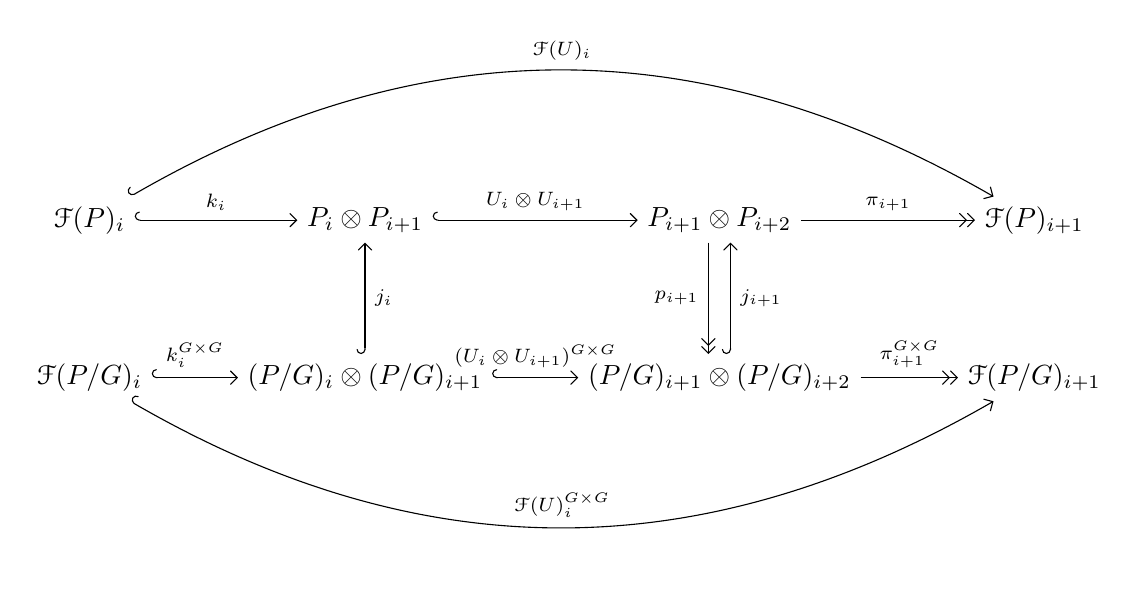
\begin{tikzpicture}[baseline=(current  bounding  box.center)]
\node (a) at (0,0) {$\mathcal F(P)_i$};
\node (b) at (3.5,0) {$P_i \otimes P_{i+1}$};
\node (c) at (8,0) {$P_{i+1} \otimes P_{i+2} $};
\node (d) at (12,0) {$\mathcal F(P)_{i+1}$};
\node (e) at (0,-2) {$\mathcal F(P/G)_i$};
\node (f) at (3.5,-2) {$(P/G)_i \otimes (P/G)_{i+1}$};
\node (g) at (8,-2) {$(P/G)_{i+1} \otimes (P/G)_{i+2} $};
\node (h) at (12,-2) {$\mathcal F(P/G)_{i+1}$};
\path[right hook->,font=\scriptsize,>=angle 90]
([xshift= 4pt]g.north) edge node[right] {$j_{i+1}$} ([xshift= 4pt]c.south)
(a) edge node[above]{$k_i$} (b)
(b) edge node[above]{$U_i\otimes U_{i+1}$} (c)
(e) edge node[above]{$k_i^{G\times G}$}(f)
(f) edge node[above] {$(U_i \otimes U_{i+1})^{G\times G}$} (g)
(f) edge node[right] {$j_{i}$} (b)
(a) edge [bend left] node[above] {$\mathcal F(U)_i$} (d)
(e) edge [bend right] node[above] {$\mathcal F(U)^{G\times G}_i$} (h)
;
\path[->>,font=\scriptsize,>=angle 90]
([xshift= -4pt]c.south) edge node[left] {$p_{i+1}$} ([xshift= -4pt]g.north)
(c) edge node[above] {$\pi_{i+1}$}(d)
(g) edge node[above] {$\pi_{i+1}^{G\times G}$} (h)
;
\end{tikzpicture}
\end{equation}
\end{rem}

\begin{lem}
\label{one_sided_inverse}
The map $p_i$ is a left inverse for $j_i.$ That is, $p_{i}\circ j_{i} = \id.$
\end{lem}
\begin{proof}
For $Gx \otimes Gy \in (P/G)_{i} \otimes (P/G)_{i+1},$ we have
\begin{align*}
	 p_{i}\circ j_{i}(Gx \otimes Gy) &= p_{i}(\frac{1}{|G|}\sum_{g \in G}^{} gx\otimes \frac{1}{|G|}\sum_{h\in G}^{}hy)\\
	 &= \frac{1}{|G|}\sum_{g \in G}^{} Gx\otimes \frac{1}{|G|}\sum_{h\in G}^{}Gy\\
	 &= Gx \otimes Gy
\end{align*}
\end{proof}



\begin{lem}
\label{center_commutes}
 The central square commutes. That is, $j_{i+1} \circ (U_i \otimes U_{i+1})^{G\times G} = (U_i \otimes U_{i+1})\circ j_i.$
\end{lem}
\begin{proof}
By definition, $(U_i \otimes U_{i+1})^{G\times G} = p_{i+1}\circ(U_i \otimes U_{i+1})\circ j_i.$ Therefore, we have $j_{i+1} \circ (U_i \otimes U_{i+1})^{G\times G} = j_{i+1}\circ p_{i+1}\circ(U_i \otimes U_{i+1})\circ j_i.$

So, in order to complete the lemma, it suffices to show that $j_{i+1} \circ p_{i+1}|_{\im((U_i \otimes U_{i+1})\circ j_i)}= \id|_{\im((U_i \otimes U_{i+1})\circ j_i)}.$ Indeed, any element $v \in \im((U_i \otimes U_{i+1})\circ j_i)$ must be of the form 
\begin{align*}
	v=\sum_{x\otimes y}^{}c_{x\otimes y}\left(\frac{1}{|G|}\sum_{g \in G}^{} gx\otimes \frac{1}{|G|}\sum_{h\in G}^{}hy\right).
\end{align*}

In order to show 
\begin{align*}
	j_{i+1} \circ p_{i+1}|_{\im((U_i \otimes U_{i+1})\circ j_i)}= \id|_{\im((U_i \otimes U_{i+1})\circ j_i)},
\end{align*} it suffices to check it on a basis. That is, we only have to show

\begin{align*}
	j_{i+1} \circ p_{i+1}\left(\frac{1}{|G|}\sum_{g \in G}^{} gx\otimes \frac{1}{|G|}\sum_{h\in G}^{}hy\right)= \frac{1}{|G|}\sum_{g \in G}^{} gx\otimes \frac{1}{|G|}\sum_{h\in G}^{}hy,
\end{align*}  or equivalently
\begin{align*}
	j_{i+1} \circ p_{i+1}\left(\sum_{g \in G}^{} gx\otimes \sum_{h\in G}^{}hy\right)= \sum_{g \in G}^{} gx\otimes \sum_{h\in G}^{}hy.
\end{align*}
However,
\begin{align*}
	j_{i+1} \circ p_{i+1}\left(\sum_{g \in G}^{} gx\otimes \sum_{h\in G}^{}hy\right)&= j_{i+1}\left(\sum_{g \in G}^{} Gx\otimes \sum_{h\in G}^{}Gy\right)\\
	&= j_{i+1}\left(|G| \cdot Gx\otimes |G|\cdot Gy\right)\\
	&= \frac{1}{|G|} \sum_{g \in G}^{}|G|gx\otimes \frac{1}{|G|}\sum_{h\in G}^{}|G|hy\\
	&= \sum_{g \in G}^{}gx\otimes\sum_{h\in G}^{}hy
\end{align*}
\end{proof}

\begin{lem}
If $\mathcal F(U)_i$ is injective, then $\ker(\pi_i)|_{\im((U_i \otimes U_{i+1})\circ k_i)}=0.$
\end{lem}
\begin{proof}
Since $\mathcal F(U)_i$ is injective, $\ker \mathcal F(U)_i  = 0.$ Therefore, since $\mathcal F(U)_i = \pi_i \circ (U_i\otimes U_{i+1}) k_i,$ we have $\ker(\pi_i)|_{\im((U_i \otimes U_{i+1})\circ k_i)}=0.$
\end{proof}

\begin{lem}
\label{no_pi_kernel}
If $\mathcal F(U)_i,$ are injective, then $\ker \pi_{i+1} \cap \im((U\otimes U)\circ j_i\circ k^{G\times G}_i)=0.$
\end{lem}
\begin{proof}
Any element $v \in \im((U\otimes U)\circ j_i\circ k^{G\times G}_i)$ can be written in the form 
\begin{align*}
	v=\sum_{x\otimes y}^{}c_{x\otimes y}\left(\frac{1}{|G|}\sum_{g \in G}^{} gx\otimes \frac{1}{|G|}\sum_{h\in G}^{}hy\right).
\end{align*}

Therefore, if $v \in \ker \pi_{i+1},$ we must have $\pi_{i+1}\left(\frac{1}{|G|}\sum_{g \in G}^{} gx\otimes \frac{1}{|G|}\sum_{h\in G}^{}hy\right) = 0$ for all pairs $(x,y),$ such that $x \in Gx,y \in Gy,$ because distinct orbits are disjoint. Hence, it suffices to show that we cannot have $\pi_{i+1}\left(\frac{1}{|G|}\sum_{g \in G}^{} gx\otimes \frac{1}{|G|}\sum_{h\in G}^{}hy\right) = 0.$

We know that if $\frac{1}{|G|}\sum_{g \in G}^{} gx\otimes \frac{1}{|G|}\sum_{h\in G}^{}hy \in \im((U\otimes U)\circ j_i\circ k^{G\times G}_i),$ then there must exist some $x \in Gx,y \in Gy$ for which $x \lessdot y.$ However, this implies that $x \otimes y \in Supp\left(\pi_{i+1}\left(\frac{1}{|G|}\sum_{g \in G}^{} gx\otimes \frac{1}{|G|}\sum_{h\in G}^{}hy\right)\right),$ and so in particular $\pi_{i+1}\left(\frac{1}{|G|}\sum_{g \in G}^{} gx\otimes \frac{1}{|G|}\sum_{h\in G}^{}hy\right) \neq 0.$
\end{proof}

\begin{lem}
\label{pi_gg_subset}
We have $\ker \left(\pi^{G\times G}_{i+1}\circ p_{i+1}\right) \cap \im((U\otimes U)\circ j_i\circ k^{G\times G}_i)\subset \ker \pi_{i+1} \cap \im((U\otimes U)\circ j_i\circ k^{G\times G}_i)$
\end{lem}
\begin{proof}
Once, again, starting with an arbitrary $v \in \im((U\otimes U)\circ j_i\circ k^{G\times G}_i),$ we can write
\begin{align*}
	v=\sum_{x\otimes y}^{}c_{x\otimes y}\left(\frac{1}{|G|}\sum_{g \in G}^{} gx\otimes \frac{1}{|G|}\sum_{h\in G}^{}hy\right).
\end{align*}
where $x \lessdot y,$ for all $x \otimes y$ in the support of the above sum. The aim is to show that $v \in \ker \pi \implies v \in \ker (\pi^{G\times G}_i \circ p_i)$ Since distinct $G$ orbits are disjoint, we can assume $v = \frac{1}{|G|}\sum_{g \in G}^{} gx\otimes \frac{1}{|G|}\sum_{h\in G}^{}hy.$ In this case, if $v \in \ker \pi,$ this means $x \not \lessdot y$ for any $x \in Gx,y \in Gy.$ But this means $Gx \not \lessdot Gy,$ and so $v \in \ker (\pi^{G\times G}_i \circ p_i).$ 
\end{proof}

\begin{cor}
\label{no_pi_gg_kernel}
If $\mathcal F(U)_i,$ are injective, then $\ker (\pi^{G\times G}_{i+1}\circ p_{i+1}) \cap \im((U\otimes U)\circ j_i\circ k^{G\times G}_i)=0.$
\end{cor}
\begin{proof}
By ~\ref{pi_gg_subset}, we know $\ker (\pi^{G\times G}_{i+1}\circ p_{i+1}) \cap \im((U\otimes U)\circ j_i\circ k^{G\times G}_i) \subset \ker \pi_{i+1} \cap \im((U\otimes U)\circ j_i\circ k^{G\times G}_i).$ But by ~\ref{no_pi_kernel} we know  $\ker \pi_{i+1} \cap \im((U\otimes U)\circ j_i\circ k^{G\times G}_i)=0.$ Therefore, $\ker (\pi^{G\times G}_{i+1}\circ p_{i+1}) \cap \im((U\otimes U)\circ j_i\circ k^{G\times G}_i)=0.$
\end{proof}

\begin{lem}
\label{injective_chain}
If $\mathcal F(U)_i,U_i,U_{i+1}$ are injective, then so is $\pi^{G\times G}_{i+1}\circ p_{i+1}\circ(U_i\otimes U_{i+1})\circ j_i\circ k^{G\times G}_i.$
\end{lem}
\begin{proof}
Since $U_i,U_{i+1}$ are both injective, $U_i \otimes U_{i+1}$ is as well. It is always the case that $j_i,k^{G\times G}_i$ are injective. Therefore, $(U_i\otimes U_{i+1})\circ j_i\circ k^{G\times G}_i$ is injective. In order to show $\pi^{G\times G}_{i+1}\circ p_{i+1}\circ(U_i\otimes U_{i+1})\circ j_i\circ k^{G\times G}_i$ is injective, it suffices to show that $\ker (\pi^{G\times G}_{i+1}\circ p_{i+1}) \cap \im((U\otimes U)\circ j_i\circ k^{G\times G}_i)=0,$ which is precisely true by ~\ref{no_pi_gg_kernel}
\end{proof}

\begin{lem}
\label{two_equivalent_paths}
We have an equality of linear transformations $\pi^{G\times G}_{i+1}\circ p_{i+1}\circ(U_i\otimes U_{i+1})\circ j_i\circ k^{G\times G}_i = \mathcal F(U)_i.$
\end{lem}
\begin{proof}
By ~\ref{center_commutes}, we have
\begin{align*}
	\pi^{G\times G}_{i+1}\circ p_{i+1}\circ(U_i\otimes U_{i+1})\circ j_i\circ k^{G\times G}_i = \pi^{G\times G}_{i+1}\circ p_{i+1}\circ j_{i+1}\circ(U_i\otimes U_{i+1})^{G\times G}\circ k^{G\times G}_i.
\end{align*}

Then, by ~\ref{one_sided inverse}, we obtain
\begin{align*}
	\pi^{G\times G}_{i+1}\circ p_{i+1}\circ j_{i+1}\circ(U_i\otimes U_{i+1})^{G\times G}\circ k^{G\times G}_i &= \pi^{G\times G}_{i+1}\circ(U_i\otimes U_{i+1})^{G\times G}\circ k^{G\times G}_i\\
	&= \mathcal F(U)_i
\end{align*}
Therefore,
\begin{align*}
	\pi^{G\times G}_{i+1}\circ p_{i+1}\circ(U_i\otimes U_{i+1})\circ j_i\circ k^{G\times G}_i = \mathcal F(U)_i.
\end{align*}
\end{proof}

\begin{thm}
\label{injectivity_thm}
If $\mathcal F(U)_i,U_i,U_{i+1}$ are injective, then $\mathcal F(U)_i$ is injective.
\end{thm}
\begin{proof}
By ~\ref{injective_chain}, we know $\pi^{G\times G}_{i+1}\circ p_{i+1}\circ(U_i\otimes U_{i+1})\circ j_i\circ k^{G\times G}_i$ is injective. But by ~\ref{two_equivalent_paths}, $\pi^{G\times G}_{i+1}\circ p_{i+1}\circ(U_i\otimes U_{i+1})\circ j_i\circ k^{G\times G}_i = \mathcal F(U)_i.$ Therefore, $\mathcal F(U)_i$ is injective.
\end{proof}

\section{The object $\mathcal F(B_n).$}

\end{document}